\begin{minipage}{.6\linewidth}
	\vspace{-4cm}
	\item A polia dupla consiste de duas peças que estão fixadas uma a outra. Ela tem uma massa de \SI{25}{\kilogram} e um
	raio de giração em relação a seu centro $k_{0}=\SI{.24}{\meter}$. Se ela gira a uma velocidade angular de \SI{20}{\radian/\second},
	no sentido horário, determine a energia cinética do sistema.
	Suponha que nenhum dos cabos deslize sobre a polia.
\end{minipage}
\begin{minipage}{.4\linewidth}
	\begin{flushright}
		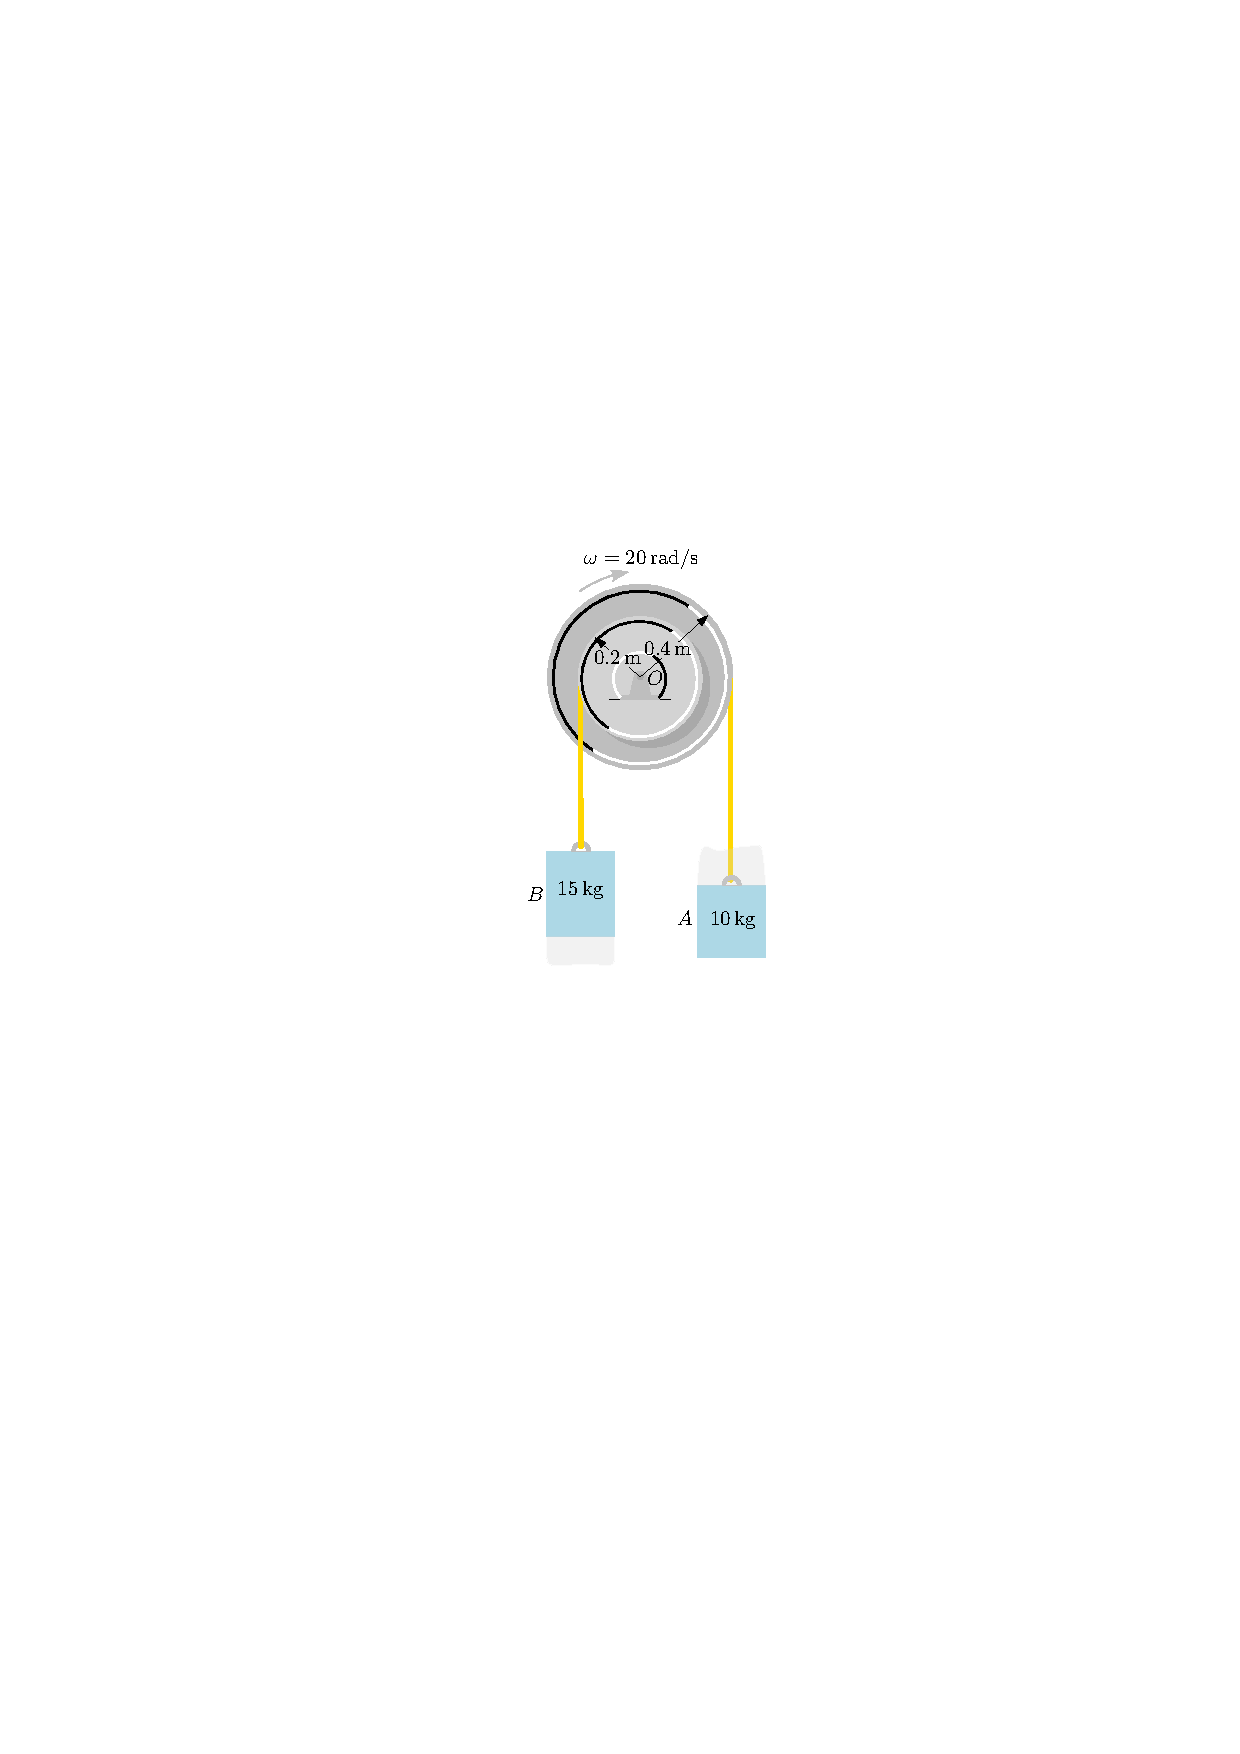
\includegraphics[scale=1.2]{../../images/draw_1}
	\end{flushright}
\end{minipage}